\documentclass[a4paper]{ctexart}
\usepackage[top=2.3cm,bottom=2cm,left=1.7cm,right=1.7cm]{geometry} 
\usepackage{amsmath} 
\usepackage{booktabs}
\usepackage{amsthm}
\usepackage{longtable} 
\usepackage{graphicx}
\usepackage{subfigure}
\usepackage{caption}
\usepackage{fontspec}
\usepackage{titlesec}
\usepackage{fancyhdr}
\def\degree{$^{\circ}$}
\def\mm{\mathrm{mm}}
\def\cm{\mathrm{cm}}
\def\nm{\mathrm{nm}}
\def\kpa{\mathrm{kpa}}
\def\V{\mathrm{V}}
\def\m{\mathrm{m}}
\def\g{\mathrm{g}}
\def\Pa{\mathrm{Pa}}
\def\s{\mathrm{s}}
\title{\textbf{刚体转动实验}}
\author{王崇斌 1800011716}
\date{}
\makeatletter %使\section中的内容左对齐
\renewcommand{\section}{\@startsection{section}{1}{0mm}
	{-\baselineskip}{0.5\baselineskip}{\bf\leftline}}
\makeatother
\begin{document}
	\pagestyle{fancy}
	\lhead{普通物理实验报告} 
	\chead{}
	\rhead{}
	\maketitle
	\thispagestyle{fancy}
    \section{\large{数据与处理}}
    \subsection{实验一}
    \par 
    实验一中,我们固定$m_{0}$位置于$(5,5^{'})$,固定塔轮的半径为2.5cm,固定砝码托距离地面
    的距离为85.2cm。改变砝码的质量,测量下落时间。
    \begin{table}[htbp]
        \centering
        \caption{实验一测量数据表}
        \begin{tabular}{ccccccc}
            \toprule[1.5pt]
            $m(\g)$ & $t_{1}(\s)$ & $t_{2}(\s)$ & $t_{3}(\s)$ & $\bar{t}(\s)$ & $\frac{1}{t^{2}}(\times 10^{-3}s^{-2})$ & $\Delta \frac{1}{t^{2}}(\times 10^{-3}s^{-2})$\\
            \midrule
            5.00 & 19.31 & 19.19 & 19.60 & 19.37 & 2.66 &  \\ 
            10.00 & 12.06 & 12.00 & 12.03 & 12.03 & 6.91 & 4.25 \\
            15.00 & 9.47 & 9.37 & 9.44 & 9.43 & 11.2 & 4.39 \\
            20.00 & 7.96 & 8.00 & 8.00 & 7.99 & 15.7 & 4.5 \\
            25.00 & 7.16 & 7.12 & 7.06 & 7.11 & 19.8 & 4.1 \\
            30.00 & 6.41 & 6.46 & 6.40 & 6.42 & 24.3 & 4.5 \\
            35.00 & 5.87 & 5.90 & 5.94 & 5.90 & 28.7 & 4.4 \\
            40.00 & 5.50 & 5.50 & 5.50 & 5.50 & 33.0 & 4.3 \\ 
            \bottomrule[1.5pt]
        \end{tabular}
    \end{table}
    \begin{figure}[htbp]
        \centering
        \includegraphics[scale = 0.48]{1_curve.eps}
        \caption{实验一中$\frac{1}{t^{2}}-m$关系图}
    \end{figure}
    \par 
    我们做出$\frac{1}{t^(2)}-m$关系图,可以看出两者有非常好的线性关系。$k = 0.896\;\mathrm{kg^{-1} s^{-2}}$,$b = -0.00176\;\mathrm{s^{-2}}$
    $r = 0.99992$。在忽略砝码盘下落的加速度$a$,与定滑轮转动的影响,我们可以得到理论上$\frac{1}{t^{2}}-m$的
    关系式为:
    $$
    \frac{1}{t^(2)} = \frac{mgr^(2)}{2hI} - \frac{rM_{\mu}}{2hI}
    $$
    从理论关系上可以看两者为线性关系,说明理论与实验符合地非常好,同时我们注意到摩擦力矩一定是正的,
    这也与实验数据地拟合图中直线截距为负相吻合。那么我们就可以根据斜率的表达式计算出转动惯量:
    $$
    I = \frac{gr^{2}}{2hk} = 4.01\times 10^{-3} \mathrm{kg m^{2}}
    $$
    \subsection{实验二}
    \par 
    固定$m_{0}$的位置于$(5,5^{'})$,维持砝码的质量为20g,固定砝码托下落的距离$h=85.2\cm$,
    改变塔轮半径测量下落时间。
    \begin{table}[htbp]
        \centering
        \caption{实验二测量数据表}
        \begin{tabular}{ccccccc}
            \toprule[1.5pt]
            $r(cm)$ & $t_{1}(\s)$ & $t_{2}(\s)$ & $t_{3}(\s)$ & $\bar{t}(\s)$ & $\frac{1}{rt^(2)}(m^{-1}s^(-2))$ & $\Delta \frac{1}{rt^(2)}(m^{-1}s^(-2))$ \\
            \midrule
            1.00 & 21.69 & 21.50 & 21.53 & 21.57 & 0.215 & \\
            1.50 & 13.72 & 13.69 & 13.59 & 13.67 & 0.375 & 0.142 \\
            2.00 & 10.09 & 10.07 & 10.18 & 10.11 & 0.489 & 0.132 \\
            2.50 & 8.03 & 8.07 & 8.00 & 8.03 & 0.620 & 0.131 \\
            3.00 & 6.56 & 6.66 & 6.69 & 6.64 & 0.757 & 0.137 \\
            \bottomrule[1.5pt]
        \end{tabular}
    \end{table}
    \begin{figure}[htbp]
        \centering
        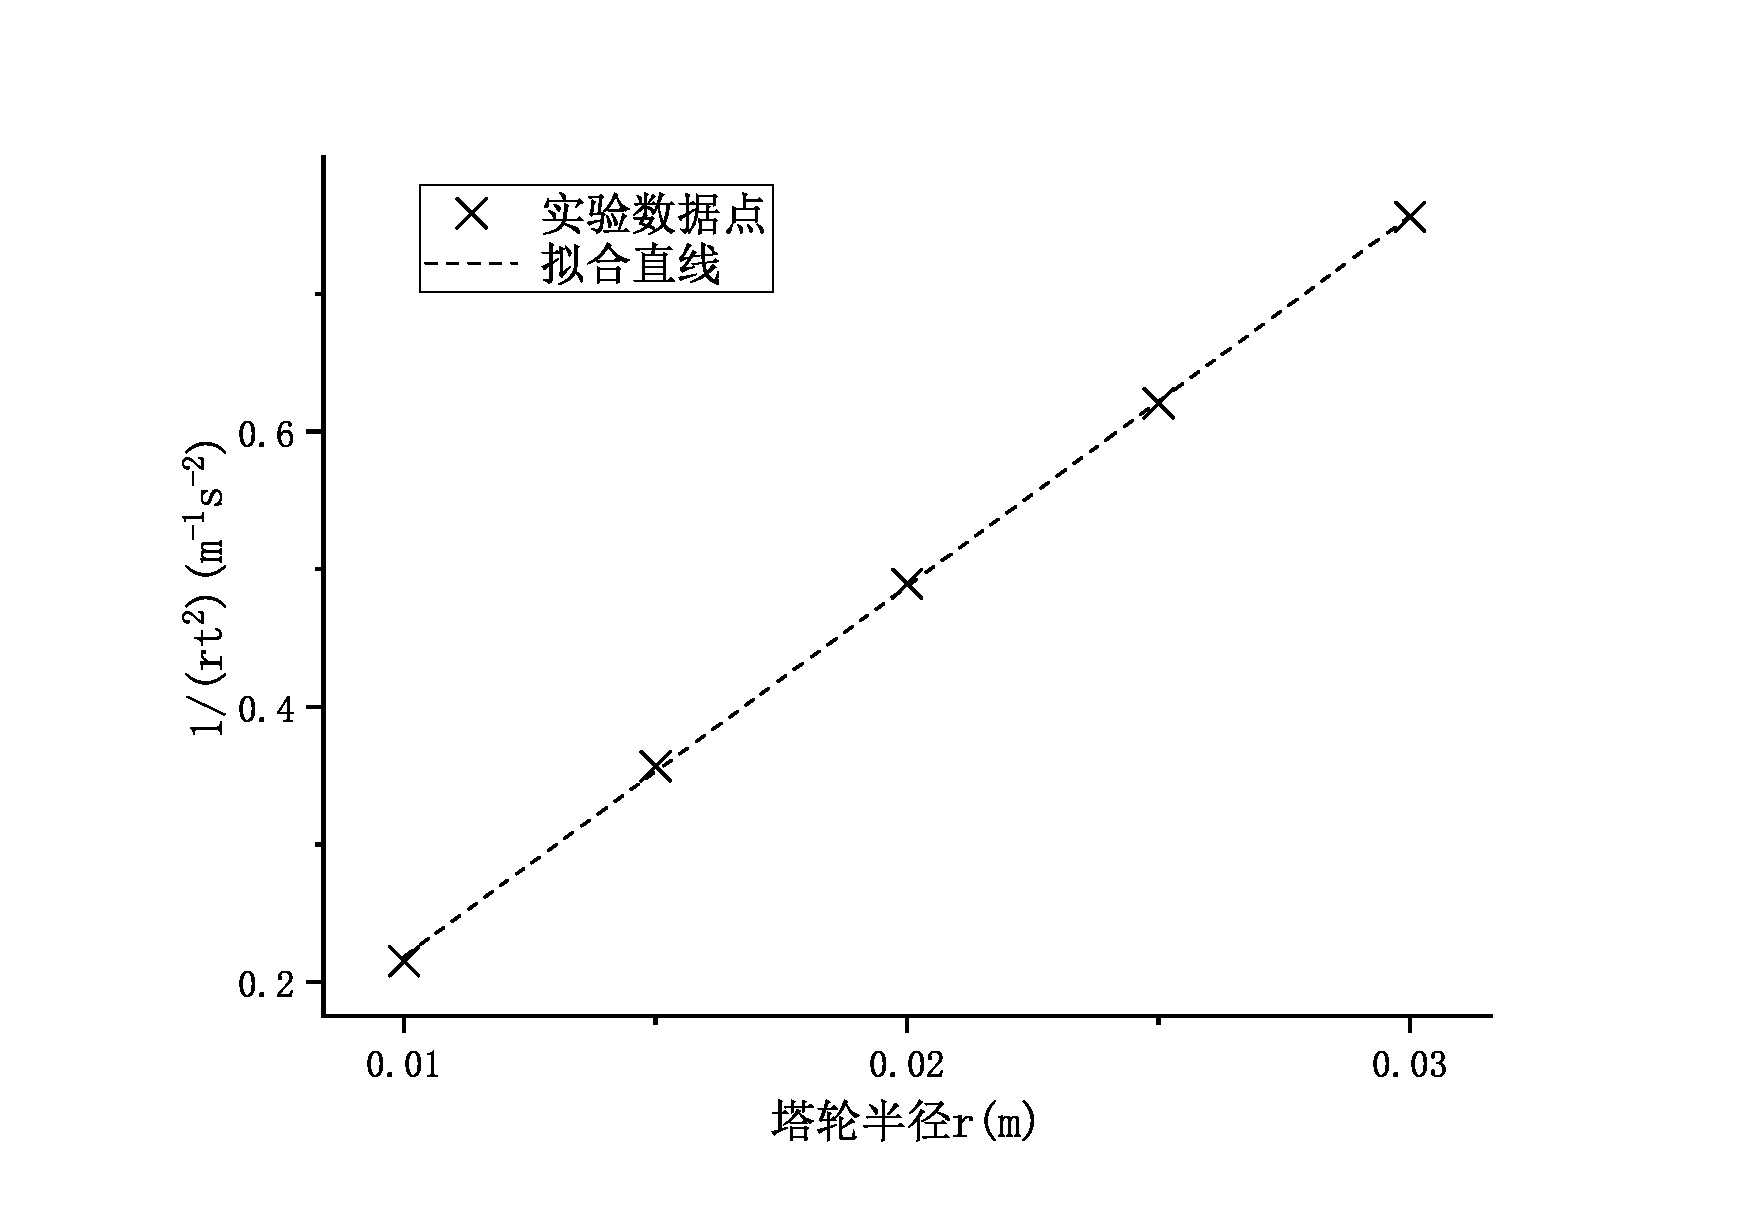
\includegraphics[scale=0.48]{2_curve.eps}
        \caption{实验一中$\frac{1}{rt^{2}}-m$关系图}
    \end{figure}
    \par 
    我们做出$\frac{1}{rt^{2}}-m$的关系图,可以看出两者呈很好的线性关系。$k = 26.92\;\mathrm{m^{-2}s^{-2}},\;\; b = -0.05087\;\mathrm{m^{-1}s^{-2}}$
    $r = 0.9998$。在忽略砝码托下落加速度的情况下,我们可以通过理论得到两者之间的关系为:
    $$
    \frac{1}{rt^{2}} = \frac{mg}{2hI}r - \frac{M_{\mu}}{2hI}
    $$
    \par 
    理论上两者也为线性关系,说明理论与实验符合地非常好。可以根据斜率的表达式计算出转动惯量为:
    $$
    I = \frac{mg}{2hk} = 4.27 \times 10^{-3} \mathrm{kg m^{2}}
    $$
    \subsection{实验三}
    \par 
    维持砝码的质量为10.00g,塔轮半径为2.5cm,固定砝码托距离地面85.2cm,对称地改变$m_{0}$的位置,
    测量下落时间。表中$x$为两个$m_{0}$到中心转轴圆柱体边缘的距离。测得两个$m_{0}$的质量分别为88.18g,80.45g。
    \begin{table}[htbp]
        \centering
        \caption{实验三测量数据表}
        \begin{tabular}{ccccccc}
            \toprule[1.5pt]
            $x_{1}(\cm)$ & $x_{2}(\cm)$ & $\bar{x}(\cm)$ & $t_{1}(\s)$ & $t_{2}(\s)$ & $t_{3}(\s)$ & $\bar{t}(\s)$\\
            \midrule
            2.096 & 2.100 & 2.098 & 7.31 & 7.28 & 7.25 & 7.28\\
            4.640 & 4.622 & 4.631 & 8.13 & 8.09 & 8.15 & 8.12\\
            7.090 & 7.128 & 7.109 & 9.31 & 9.25 & 9.34 & 9.30\\
            9.560 & 9.606 & 9.583 & 10.91 & 10.81 & 10.87 & 10.86\\
            12.070 & 12.136 & 12.013 & 12.56 & 12.54 & 12.59 & 12.56\\
            \bottomrule[1.5pt]
        \end{tabular}
    \end{table}
    \par 
    实验中发现本应质量相近的圆柱形重物$m_{0}$质量差异明显,因此不能够再使用书上提供的计算转动惯量
    的公式。在实际测量带有等分刻度的细圆柱的刻度间距后发现这个刻度是相当对称的,误差小于测量时间
    的误差,所以考虑取两个距离的平均值作为$x$,并且用两个圆柱的总质量代替$m_{0}$。
    \begin{figure}[htbp]
        \centering
        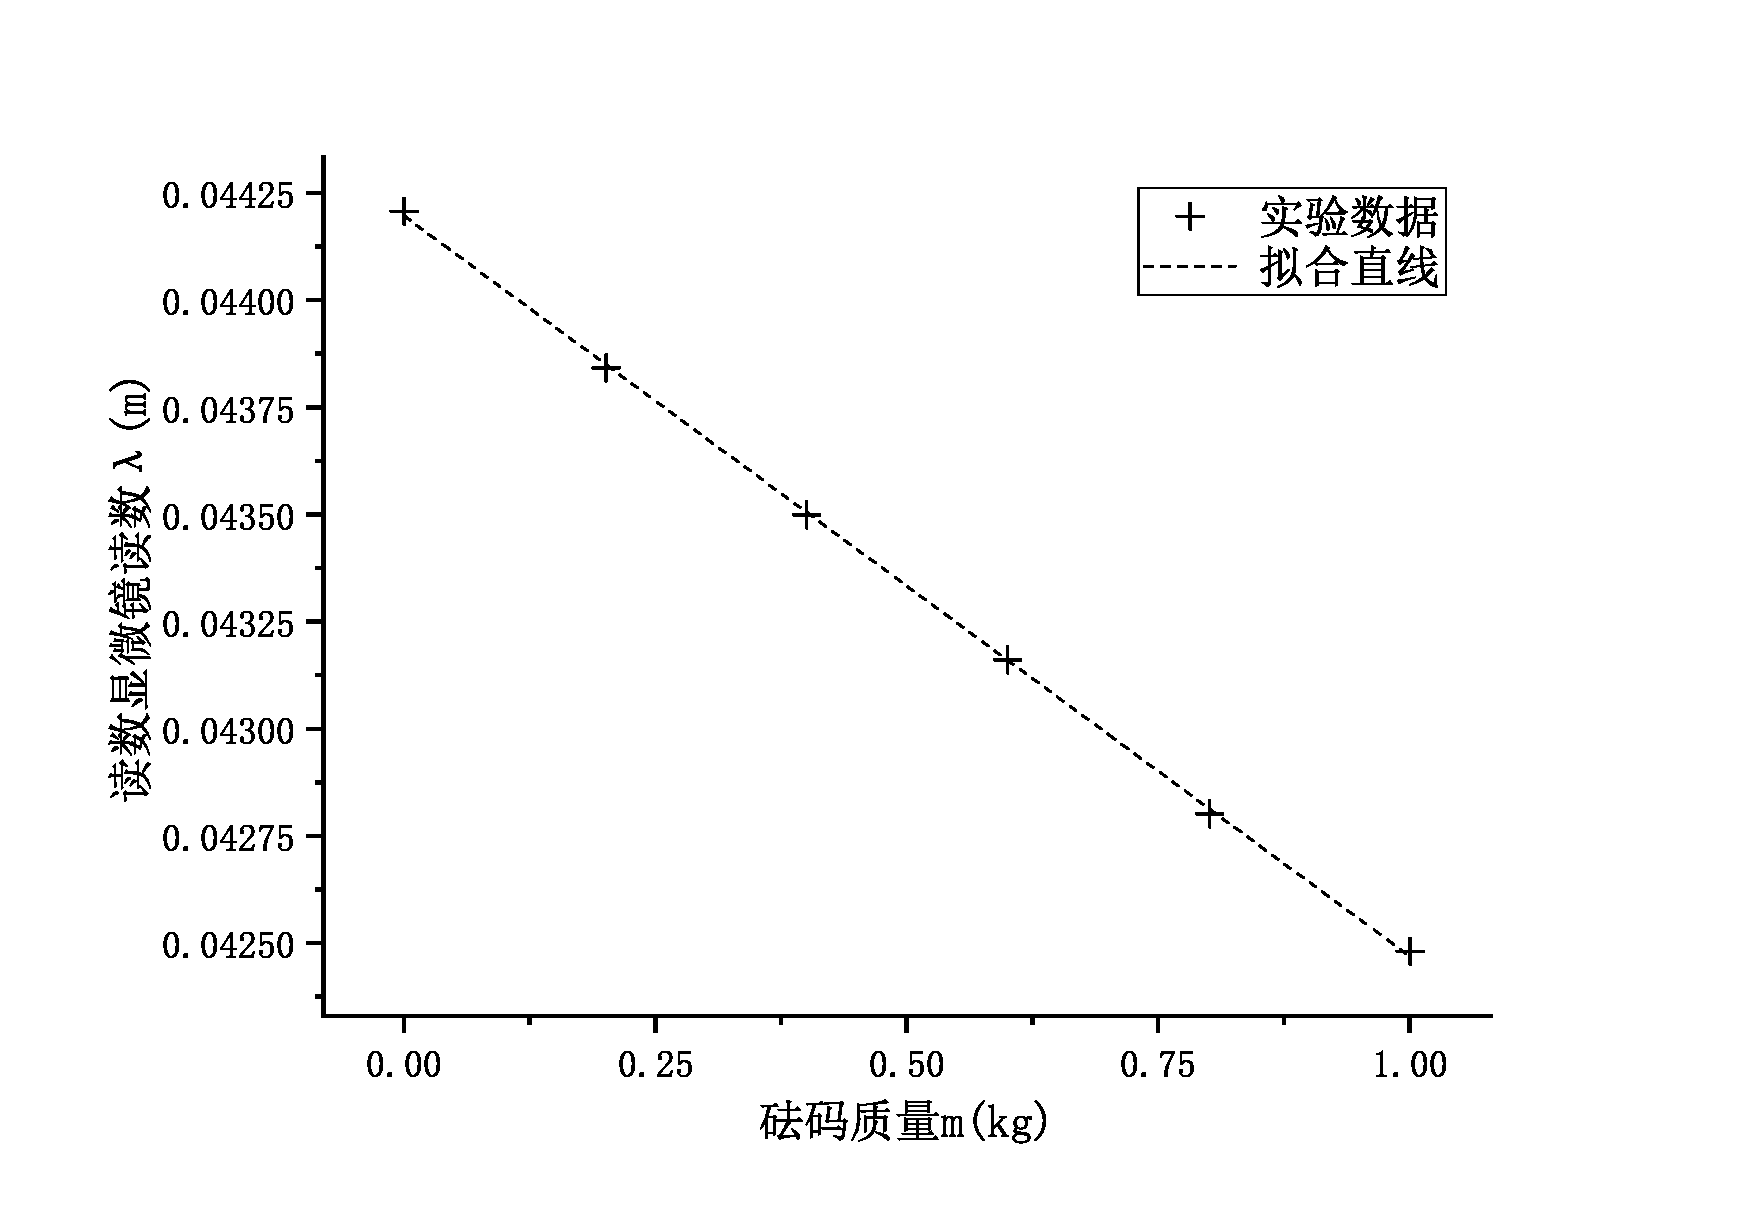
\includegraphics[scale=0.48]{3_curve.eps}
        \caption{实验三中$t^{2}-x^{2}$关系图}
    \end{figure}
    \par 
    我们首先做出$t^{2}-x^{2}$的关系图,可以看出两者有着很好的线性关系。$k = 7459\;\mathrm{m^{-2}s^{2}},\;\; b=49.5 \mathrm{s^{2}}$
    $r = 0.9998$。在忽略砝码下落加速度的情况下,我们可以通过理论(刚体转动的平行轴定理)得到两者之间的关系式为:
    $$
    t^{2} = \frac{2h}{mgr^{2}-rM_{\mu}}(m_{01} + m_{02})x^{2} + \frac{2h}{mgr^{2} - rM_{\mu}}(I_0 + I_{0c})
    $$
    \par 
    从关系式中可以看出$t^{2}-x^{2}$应呈现出严格的线性关系,这与实验结果是一致的,因此验证了平行轴定理。\\
    \\
    \section{\large{分析与讨论}}
    \subsection{如何减小实验中的随机误差与系统误差}
    \par 
    由于我们在整个实验中都忽略了定滑轮的影响,但是忽略影响是有条件的,只有当定滑轮没有质量,与轴没有摩擦时才可
    忽略其影响。那么我们在实验时应选取质量相对较轻的滑轮,并保证其与轴之间的摩擦较小。同时,在安装
    定滑轮时,应该注意线与塔轮的接触点应该与定滑轮共面,这样才能保证线与定滑轮之间的摩擦比较小,同时
    还应保证定滑轮上端与塔轮绕线处同意水平高度,这样使用塔轮半径作为力臂才是正确的。在安装整个装置时
    应该注意使塔轮与上下接触点之间的摩擦尽可能地小,但是也不能使轴有明显的相对晃动,否则就不是我们所
    研究的定轴转动的情况了。按照上面的操作就可以减小系统误差。
    \par 
    本实验中随机误差的主要来源为时间的测量,因为时间的测量带有很大的主观性。在开始计时时,我们必须保证、
    砝码托是从零开始加速的, 为此我们可以使用挡板挡住细杆,在抽出挡板的同时开始计时;同样的,我们也应该
    想办法保证下落至地面的时刻记录是准确的,应该集中注意力观察砝码的下落,并在下落快至终点时将秒表的按键
    按下一半,这样可以使得记录更准确,平行测定时间的方差更小。
    \subsection{砝码托加速度对于实验的影响}
    \par 
    若考虑砝码托下落的加速度,那么由转动定理导出的方程为:
    $$
    m\left(g-\frac{2h}{t^{2}}\right)r - M_{\mu} = \frac{2hI}{rt^{2}}
    $$
    \par 
    此时$\frac{1}{t^{2}}-m$不再呈现出严格的线性关系,具体的影响可以通过对上式进行Taylor展开
    然后讨论,我们这里只进行一个简单的讨论,即比较重力加速度与砝码托之间加速度的大小关系。我们
    选取一个最大的加速度进行计算,即实验一中的最后一组数据:
    $$
    a = \frac{2h}{t^{2}} = 0.056\;\mathrm{m/s^{2}}
    $$
    \par 
    相对于重力加速度只有千分之五,远小于时间测量的误差,因此忽略砝码托下落加速度是一个很好的近似。
\end{document}